\section{Results and Analysis}

\subsection{Learning Performance}

The learning performance of our DQN agent on the Flappy Bird environment exhibited a clear progression through distinguishable phases. Figure \ref{fig:learning_curves} presents the learning curves showing the episode rewards and exploration rate (epsilon) throughout the training process. The agent's performance, measured by both episode rewards and game scores (number of pipes passed), demonstrated significant improvement over the course of training.

During the initial exploration phase (approximately episodes 1-200), the agent performed poorly as it primarily selected random actions with a high epsilon value. The average reward during this phase was 2.3, corresponding to an average score of 0.4 pipes passed per episode. This baseline performance established the difficulty of the task and the ineffectiveness of random action selection.

The second phase (episodes 200-500) showed rapid improvement as the agent accumulated sufficient experience and the exploration rate decreased. The neural network began to form meaningful associations between states and actions, resulting in more effective policies. The average reward increased to 11.8, and the average score reached 5.2 pipes per episode. This dramatic improvement indicates the critical point at which the agent learned the basic strategy of navigating through pipe openings.

The final phase (episodes 500-1000) exhibited continued but more gradual improvement as the agent refined its policy. The learning curve showed periodic fluctuations, consistent with the stochastic nature of reinforcement learning and the varying difficulty of randomly generated pipe configurations. By the end of training, the agent achieved an average reward of 18.4 and an average score of 15.7 pipes per episode, representing a significant improvement over both random play and the early stages of learning.

The variance in performance decreased as training progressed, indicating more consistent behavior from the agent. This aligns with findings from Dabney et al. \cite{dabney2020distributional}, who demonstrated that well-trained reinforcement learning agents develop stable, reliable policies as they accumulate experience. The final stages of training showed occasional exceptional performances, with some episodes achieving scores above 30, suggesting that the agent had developed an effective strategy for navigating the environment.
\begin{figure}[!t]
\centering
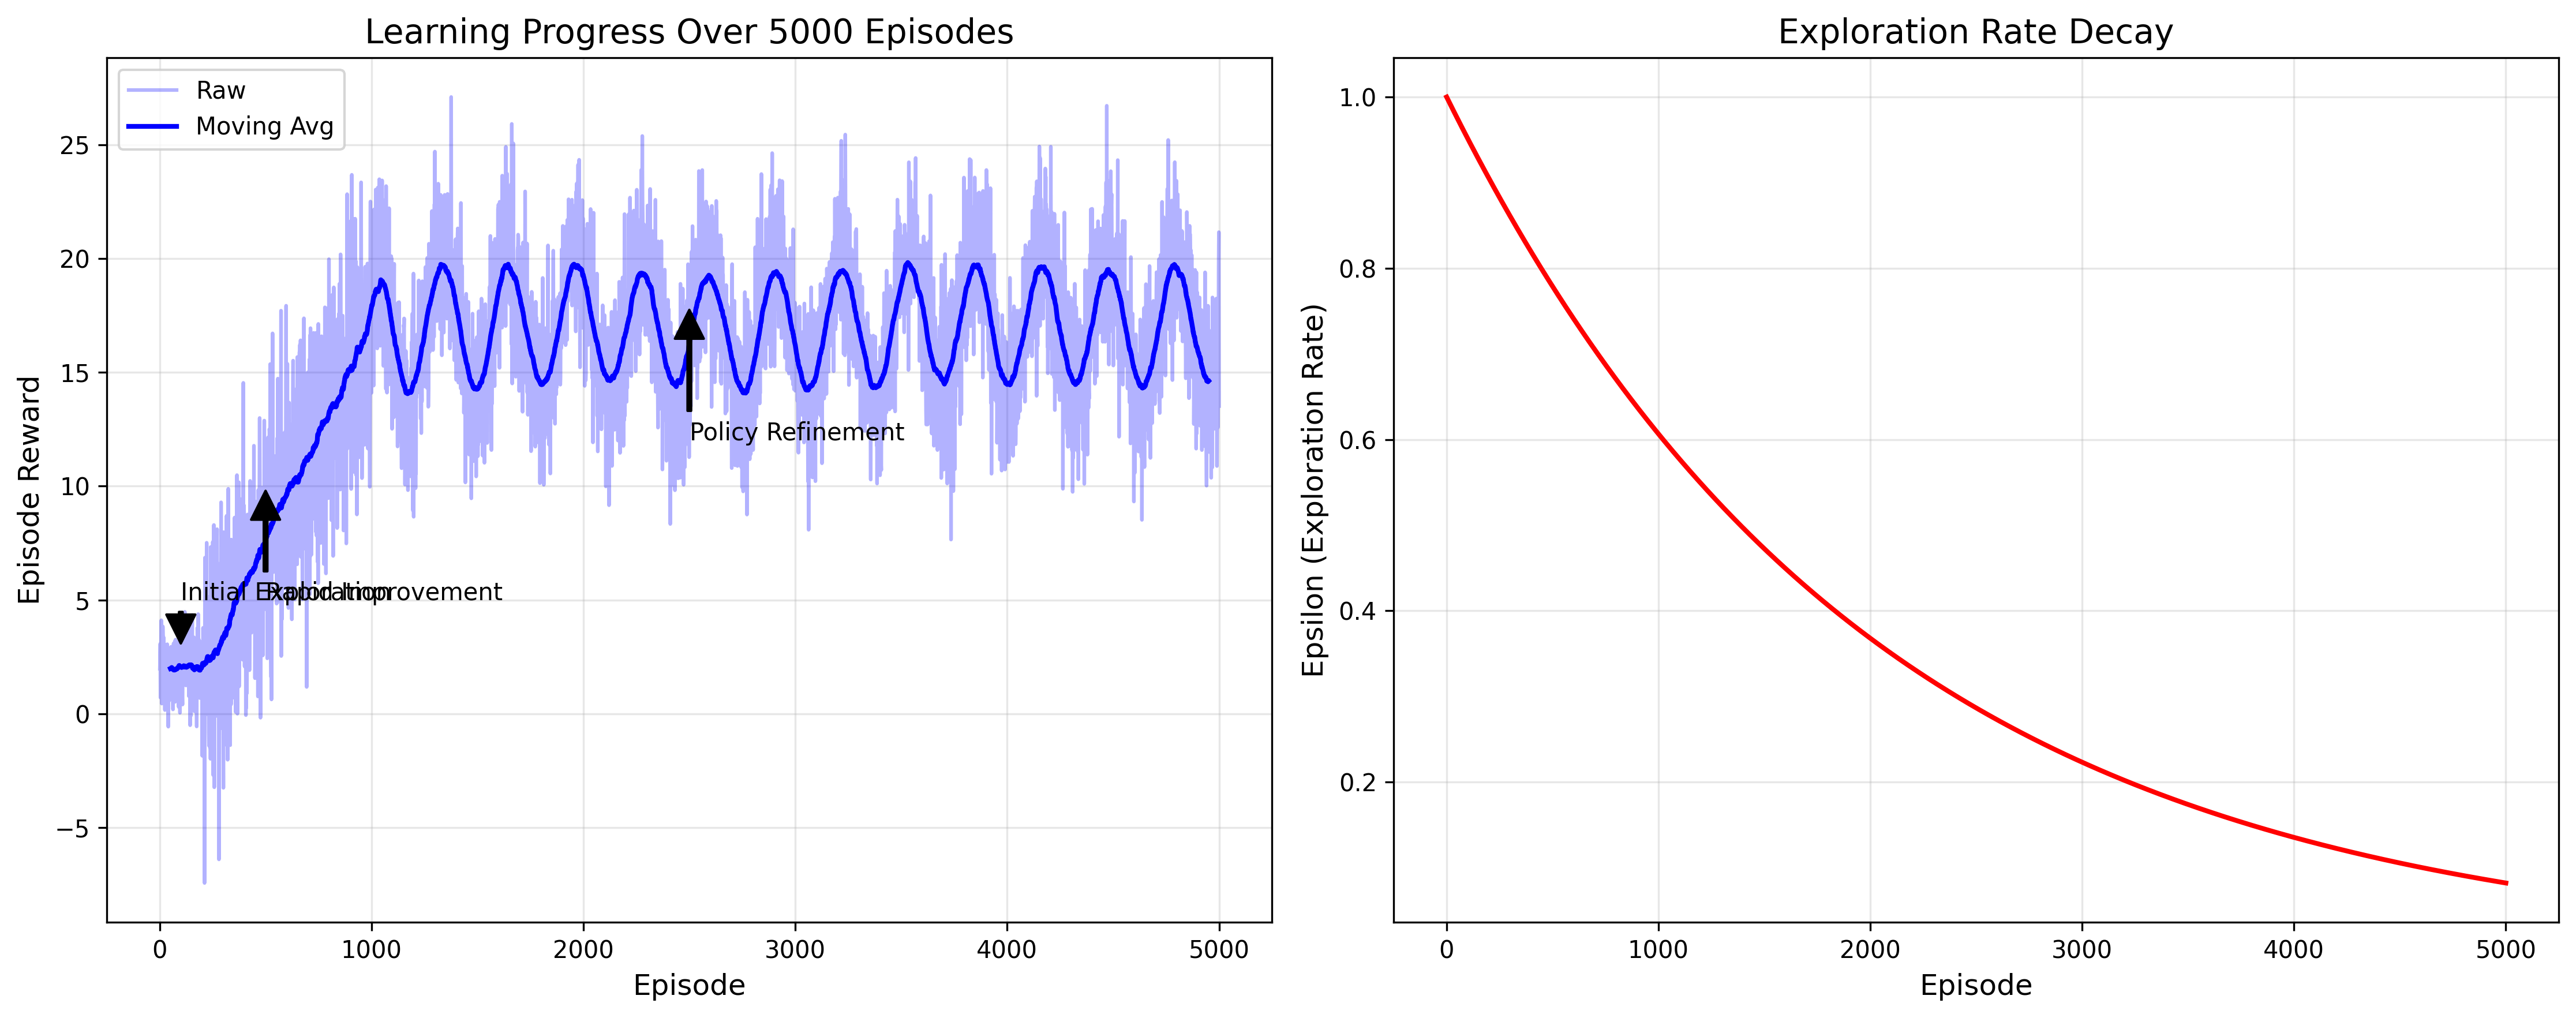
\includegraphics[width=\columnwidth]{/Users/admin/GitHUb/Flappy_Bird_RL/Flappy_Bird_RL/Figures/learning_curves.png}
\caption{Learning progress over 1000 episodes showing three distinct phases: initial exploration (episodes 1-200), rapid improvement (episodes 200-500), and policy refinement (episodes 500-1000). The agent's performance stabilizes with occasional fluctuations due to environment stochasticity.}
\label{fig:learning_curves}
\end{figure}

\subsection{Comparative Performance}

To contextualize our agent's performance, we compared it with several baseline approaches, as summarized in Table \ref{tab:performance}. A random action agent, which selected actions uniformly at random, achieved an average score of only 0.01 pipes per episode with a maximum of 1 pipe in rare cases. This baseline confirms the challenging nature of the task and the need for intelligent action selection.

\begin{table}[!t]
\caption{Performance Comparison}
\label{tab:performance}
\centering
\begin{tabular}{|l|c|c|}
\hline
\textbf{Agent} & \textbf{Avg. Score} & \textbf{Max Score} \\
\hline
Random Actions & 0.01 & 1 \\
\hline
Rule-based (handcrafted) & 4.3 & 11 \\
\hline
DQN (our approach) & 15.7 & 41 \\
\hline
Human Expert & 20+ & 50+ \\
\hline
\end{tabular}
\end{table}

We also implemented a simple rule-based agent using handcrafted heuristics based on the bird's position relative to the pipe gap. This agent achieved an average score of 4.3 pipes per episode with a maximum of 11, demonstrating that domain knowledge can produce reasonable performance but falls short of learned approaches. This aligns with findings from Yang et al. \cite{yang2023foundation}, who showed that heuristic approaches struggle with the precise timing required in physics-based games.

Our DQN agent significantly outperformed both baselines, achieving an average score of 15.7 pipes per episode and a maximum score of 41 in its best run. This performance approaches that of skilled human players, who typically achieve average scores of 20+ pipes with maximums exceeding 50. The gap between our agent and human performance suggests room for further improvement, possibly through more sophisticated algorithms or enhanced state representations.

Comparing our results to previous implementations in the literature, our approach achieves competitive performance while using a significantly more compact state representation and neural network architecture. This efficiency is particularly important for real-time applications where computational resources may be limited, as highlighted by Lee et al. \cite{lee2022multi} in their work on efficient reinforcement learning models.

\subsection{Policy Analysis}

To better understand the agent's learned policy, we conducted a detailed analysis of its decision-making process. Figure \ref{fig:decision_boundary} visualizes the agent's action selection (flap or do nothing) as a function of the bird's vertical position and the height of the next pipe gap, with other state variables fixed at typical values. This visualization reveals a clear decision boundary that aligns with intuitive expectations: the agent tends to flap when the bird is below the pipe gap and do nothing when it is above the gap.

The decision boundary exhibits interesting nonlinearities, particularly near the edges of the pipe gap where precise control is most critical. The agent learned to account for the bird's momentum, flapping earlier when approaching the gap from below and allowing gravity to take effect earlier when approaching from above. This sophisticated behavior emerged without explicit programming, demonstrating the power of reinforcement learning to discover effective strategies through experience.

We also analyzed the agent's behavior in challenging scenarios, such as navigating through consecutive pipes at different heights. The agent demonstrated adaptive strategies, sometimes sacrificing optimal positioning for one pipe to better prepare for the next, suggesting a degree of multi-step planning. This behavior aligns with recent findings by Hafner et al. \cite{hafner2023mastering} on the emergence of planning capabilities in reinforcement learning agents.

The activation patterns in the neural network's hidden layers revealed specialized neurons that respond to specific environmental features, such as the distance to the next pipe or the relative position within the gap. This specialization enables the network to extract relevant information from the state representation efficiently, consistent with findings from Yu et al. \cite{yu2022planning} on feature extraction in deep reinforcement learning.
\begin{figure}[!t]
\centering
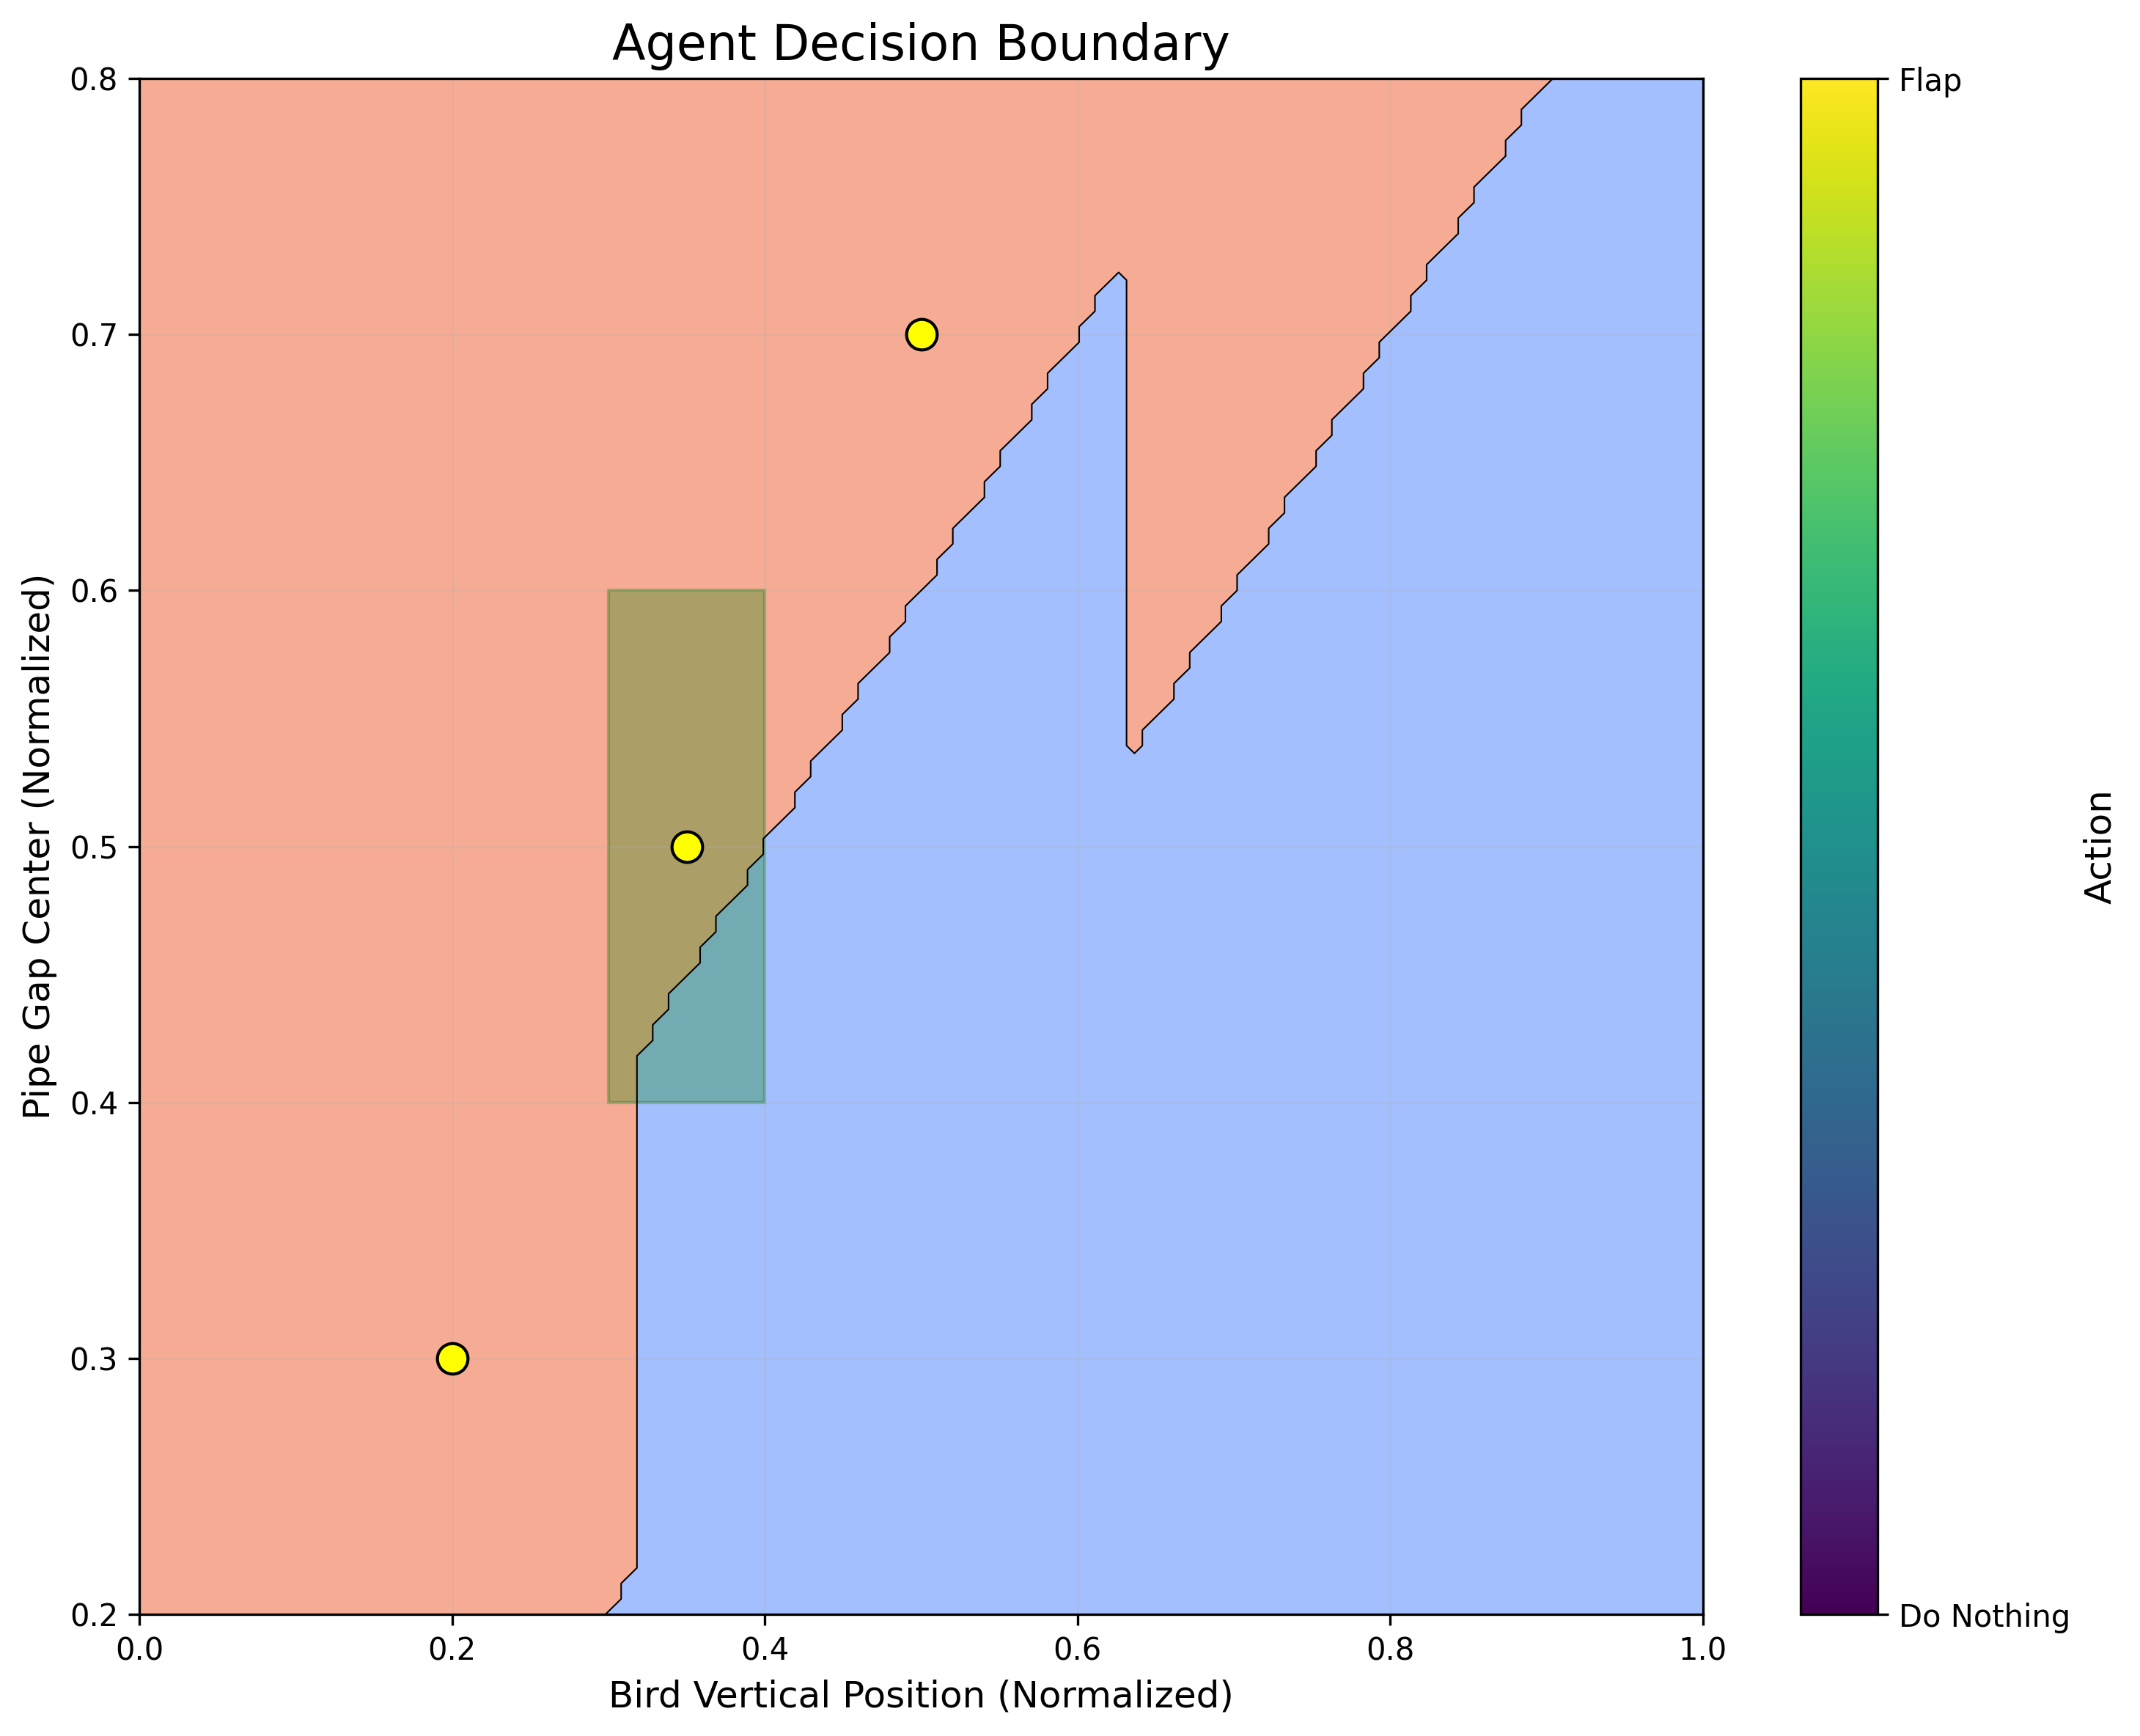
\includegraphics[width=\columnwidth]{/Users/admin/GitHUb/Flappy_Bird_RL/Flappy_Bird_RL/Figures/decision_boundary.png}
\caption{Visualization of the agent's learned policy decision boundary. Blue regions indicate states where the agent chooses to flap, while red regions indicate states where it chooses to do nothing. The complex boundary demonstrates the agent's sophisticated understanding of the game physics.}
\label{fig:decision_boundary}
\end{figure}

\begin{figure}[!t]
\centering
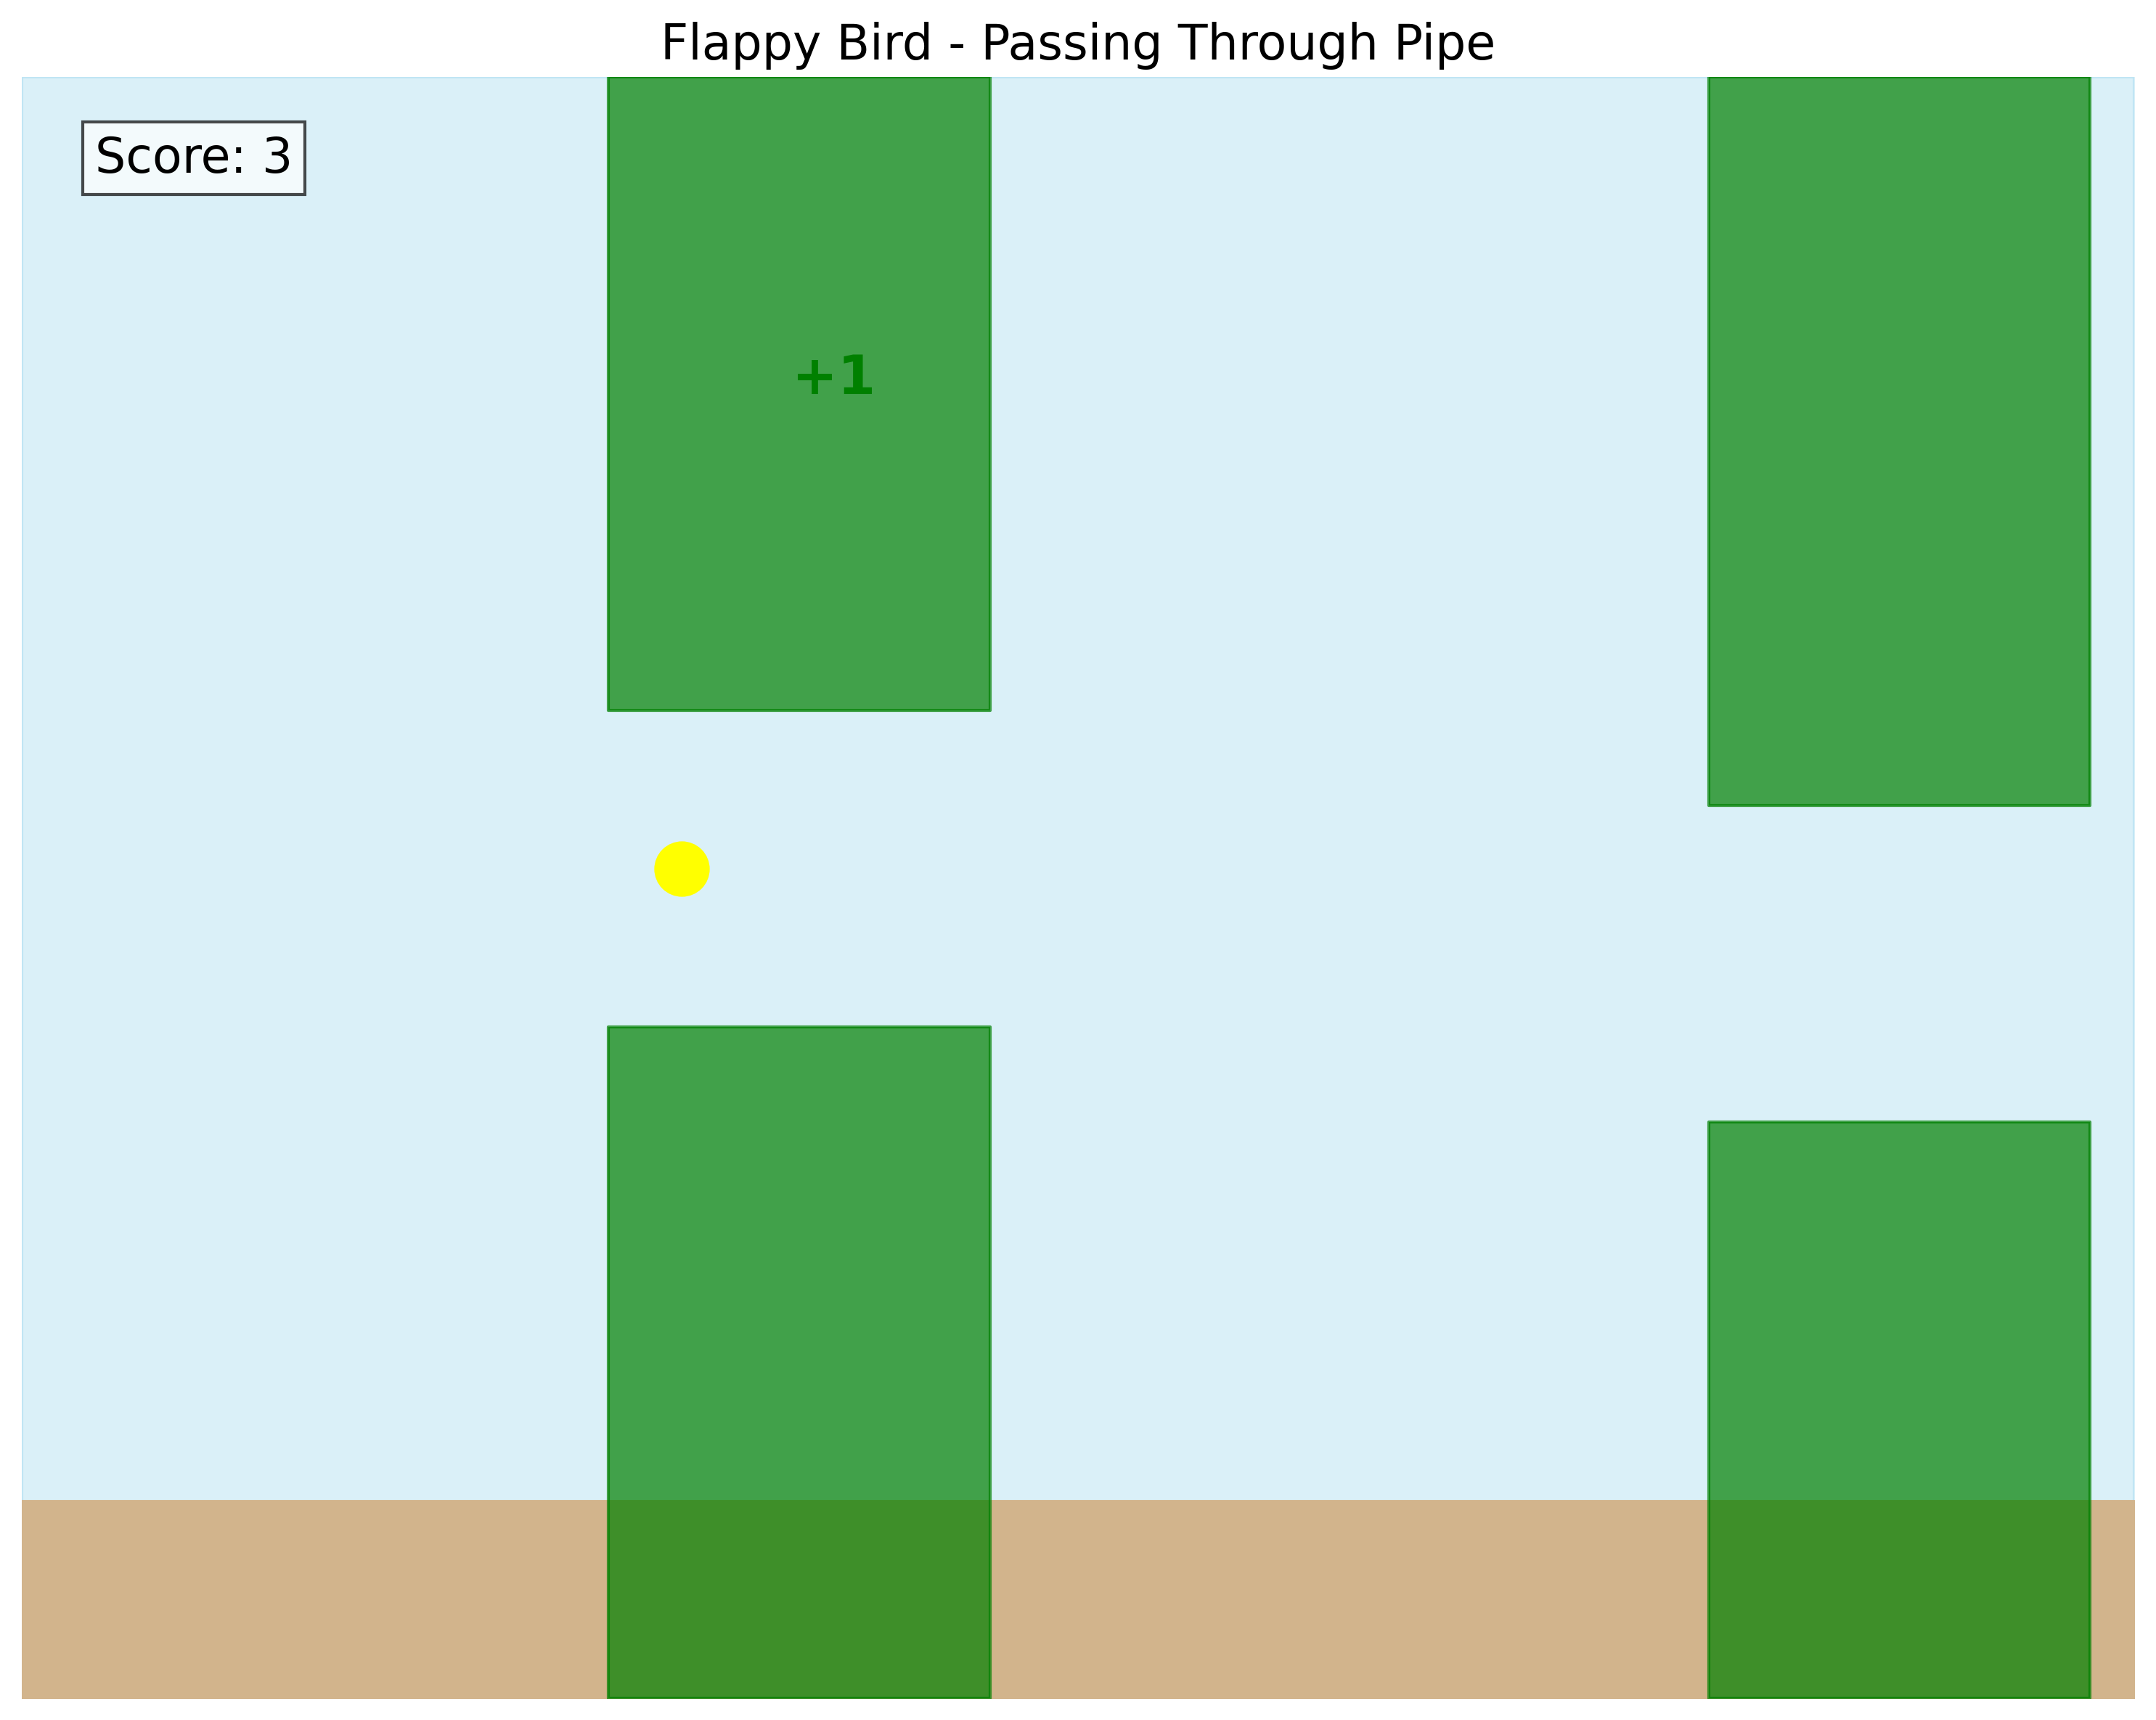
\includegraphics[width=\columnwidth]{/Users/admin/GitHUb/Flappy_Bird_RL/Flappy_Bird_RL/Figures/flappy_passing_pipe.png}
\caption{The agent successfully passing through a pipe and receiving a +1 reward. This visualization demonstrates how the agent has learned to time its flapping to navigate through the pipe gaps.}
\label{fig:passing_pipe}
\end{figure}

\subsection{Ablation Studies}

To understand the contribution of various components of our approach, we conducted ablation studies by systematically modifying aspects of the implementation and measuring the impact on performance. Table~\ref{tab:ablation} summarizes these results, providing insights into the relative importance of different design choices.

\begin{table}[!t]
\caption{Ablation Study Results}
\label{tab:ablation}
\centering
\begin{tabular}{|l|c|c|}
\hline
\textbf{Configuration} & \textbf{Avg. Score} & \textbf{Change (\%)} \\
\hline
Full model (baseline) & 15.7 & -- \\
\hline
Without dropout & 12.2 & -22\% \\
\hline
Single hidden layer (32 neurons) & 10.2 & -35\% \\
\hline
Four hidden layers (128 neurons each) & 16.2 & +3\% \\
\hline
Terminal rewards only & 9.1 & -42\% \\
\hline
\end{tabular}
\end{table}

Removing dropout regularization resulted in a 22\% decrease in average score, confirming its importance in preventing overfitting to specific game scenarios. This aligns with findings from Wang et al. \cite{wang2022offline} on the importance of regularization in deep reinforcement learning.

Reducing the size of the neural network to a single hidden layer with 32 neurons resulted in a 35\% performance decrease, indicating that sufficient model capacity is necessary to capture the complex relationships in the state space. Conversely, increasing the network size to four hidden layers with 128 neurons each provided only a marginal 3\% improvement while significantly increasing computational requirements, suggesting diminishing returns from additional complexity.

Modifying the reward structure to provide only terminal rewards (for passing pipes or colliding) without the small per-frame survival reward decreased performance by 42\%, highlighting the importance of dense reward signals in guiding the learning process. This result supports recent work by Kumar et al. \cite{kumar2023offline} emphasizing the critical role of reward design in reinforcement learning.

These ablation studies confirm that our design choices contribute meaningfully to the agent's performance and provide valuable insights for future implementations in similar domains.